%
% - Presentation Plan -
% * History
% * Maybe - mention several of the JS warts CS works around
% * Basic Operators
% * Namespaces?
% * Object literal sugar
% * Destructuring
% * String interp.
% * Classes            - Might show this live with js to coffee
% * Fat arrow
% * Method default args
% * Testing options - Show github mocha + chai?
% * Show merchinator code using JS libs
% * Show debugging merchinator code in chrome
% * Pick existing JS code and show CS version (Dashboards repo is
%   probably a good source)
%
% Compile with 'pdflatex -shell-escape coffeescript.tex'
%
\documentclass{beamer}

\usetheme{Warsaw}    

\usepackage{listings}                                   
\usepackage{hyperref}
\usepackage{graphicx}                                 
\usepackage{tabularx}
\usepackage{microtype}
\usepackage[T1]{fontenc}
\usepackage[scaled]{beramono}
\usepackage{minted}
\usepackage{multicol}

\usepackage{xcolor}

\newcommand\Small{\fontsize{5}{5.2}\selectfont}
\newcommand*\LSTfont{\Small\ttfamily\SetTracking{encoding=*}{-60}\lsstyle}

\hypersetup{colorlinks=color, linkcolor=black}
\definecolor{OliveGreen}{rgb}{0,0.6,0}
\graphicspath{{./images/}}
%
% Turn off beamer nav stuff...
%
\setbeamertemplate{navigation symbols}{}

%%
% listings does not currently support clojure...here's an attempt I
% found in a discussion thread to add clojure support.
% For the moment, this results in decent looking code. I might switch
% to minted in the future.
%
\lstdefinelanguage{clojure}%
{morekeywords={*,*1,*2,*3,*agent*,*allow-unresolved-vars*,*assert*,*clojure-version*,*command-line-args*,%
*compile-files*,*compile-path*,*e,*err*,*file*,*flush-on-newline*,*in*,*macro-meta*,%
*math-context*,*ns*,*out*,*print-dup*,*print-length*,*print-level*,*print-meta*,*print-readably*,%
*read-eval*,*source-path*,*use-context-classloader*,*warn-on-reflection*,+,-,->,->>,..,/,:else,%
<,<=,=,==,>,>=,@,accessor,aclone,add-classpath,add-watch,agent,agent-errors,aget,alength,alias,%
all-ns,alter,alter-meta!,alter-var-root,amap,ancestors,and,apply,areduce,array-map,aset,%
aset-boolean,aset-byte,aset-char,aset-double,aset-float,aset-int,aset-long,aset-short,assert,%
assoc,assoc!,assoc-in,associative?,atom,await,await-for,await1,bases,bean,bigdec,bigint,binding,%
bit-and,bit-and-not,bit-clear,bit-flip,bit-not,bit-or,bit-set,bit-shift-left,bit-shift-right,%
bit-test,bit-xor,boolean,boolean-array,booleans,bound-fn,bound-fn*,butlast,byte,byte-array,%
bytes,cast,char,char-array,char-escape-string,char-name-string,char?,chars,chunk,chunk-append,%
chunk-buffer,chunk-cons,chunk-first,chunk-next,chunk-rest,chunked-seq?,class,class?,%
clear-agent-errors,clojure-version,coll?,comment,commute,comp,comparator,compare,compare-and-set!,%
compile,complement,concat,cond,condp,conj,conj!,cons,constantly,construct-proxy,contains?,count,%
counted?,create-ns,create-struct,cycle,dec,decimal?,declare,def,definline,defmacro,defmethod,%
defmulti,defn,defn-,defonce,defprotocol,defstruct,deftype,delay,delay?,deliver,deref,derive,%
descendants,destructure,disj,disj!,dissoc,dissoc!,distinct,distinct?,do,do-template,doall,doc,%
dorun,doseq,dosync,dotimes,doto,double,double-array,doubles,drop,drop-last,drop-while,empty,empty?,%
ensure,enumeration-seq,eval,even?,every?,false,false?,ffirst,file-seq,filter,finally,find,find-doc,%
find-ns,find-var,first,float,float-array,float?,floats,flush,fn,fn?,fnext,for,force,format,future,%
future-call,future-cancel,future-cancelled?,future-done?,future?,gen-class,gen-interface,gensym,%
get,get-in,get-method,get-proxy-class,get-thread-bindings,get-validator,hash,hash-map,hash-set,%
identical?,identity,if,if-let,if-not,ifn?,import,in-ns,inc,init-proxy,instance?,int,int-array,%
integer?,interleave,intern,interpose,into,into-array,ints,io!,isa?,iterate,iterator-seq,juxt,%
key,keys,keyword,keyword?,last,lazy-cat,lazy-seq,let,letfn,line-seq,list,list*,list?,load,load-file,%
load-reader,load-string,loaded-libs,locking,long,long-array,longs,loop,macroexpand,macroexpand-1,%
make-array,make-hierarchy,map,map?,mapcat,max,max-key,memfn,memoize,merge,merge-with,meta,%
method-sig,methods,min,min-key,mod,monitor-enter,monitor-exit,name,namespace,neg?,new,newline,%
next,nfirst,nil,nil?,nnext,not,not-any?,not-empty,not-every?,not=,ns,ns-aliases,ns-imports,%
ns-interns,ns-map,ns-name,ns-publics,ns-refers,ns-resolve,ns-unalias,ns-unmap,nth,nthnext,num,%
number?,odd?,or,parents,partial,partition,pcalls,peek,persistent!,pmap,pop,pop!,pop-thread-bindings,%
pos?,pr,pr-str,prefer-method,prefers,primitives-classnames,print,print-ctor,print-doc,print-dup,%
print-method,print-namespace-doc,print-simple,print-special-doc,print-str,printf,println,println-str,%
prn,prn-str,promise,proxy,proxy-call-with-super,proxy-mappings,proxy-name,proxy-super,%
push-thread-bindings,pvalues,quot,rand,rand-int,range,ratio?,rational?,rationalize,re-find,%
re-groups,re-matcher,re-matches,re-pattern,re-seq,read,read-line,read-string,recur,reduce,ref,%
ref-history-count,ref-max-history,ref-min-history,ref-set,refer,refer-clojure,reify,%
release-pending-sends,rem,remove,remove-method,remove-ns,remove-watch,repeat,repeatedly,%
replace,replicate,require,reset!,reset-meta!,resolve,rest,resultset-seq,reverse,reversible?,%
rseq,rsubseq,second,select-keys,send,send-off,seq,seq?,seque,sequence,sequential?,set,set!,%
set-validator!,set?,short,short-array,shorts,shutdown-agents,slurp,some,sort,sort-by,sorted-map,%
sorted-map-by,sorted-set,sorted-set-by,sorted?,special-form-anchor,special-symbol?,split-at,%
split-with,str,stream?,string?,struct,struct-map,subs,subseq,subvec,supers,swap!,symbol,symbol?,%
sync,syntax-symbol-anchor,take,take-last,take-nth,take-while,test,the-ns,throw,time,to-array,%
to-array-2d,trampoline,transient,tree-seq,true,true?,try,type,unchecked-add,unchecked-dec,%
unchecked-divide,unchecked-inc,unchecked-multiply,unchecked-negate,unchecked-remainder,%
unchecked-subtract,underive,unquote,unquote-splicing,update-in,update-proxy,use,val,vals,%
var,var-get,var-set,var?,vary-meta,vec,vector,vector?,when,when-first,when-let,when-not,%
while,with-bindings,with-bindings*,with-in-str,with-loading-context,with-local-vars,%
with-meta,with-open,with-out-str,with-precision,xml-seq,zero?,zipmap
},%
   sensitive,% ???
   alsodigit=-,%
   morecomment=[l];,%
   morestring=[b]"%
  }[keywords,comments,strings]%

\lstset{
%  frame=tb,
  language=clojure,
% showstringspaces=false,
%  keepspaces=true
%  columns=fullflexible,
%  basicstyle={\LSTfont},
  numbers=none,
  numberstyle=\tiny\color{gray},
  keywordstyle=\color{blue},
  commentstyle=\color{orange},
  stringstyle=\color{OliveGreen},
%  breaklines=false,
%  breakatwhitespace=false
  tabsize=2
}


\begin{document}

\begin{frame}
  \frametitle{Intro to}
  \center{
    
\includegraphics[scale=.60]{cs-logo}
  }

  April 2014

\end{frame}

\begin{frame}
  \frametitle{History}
  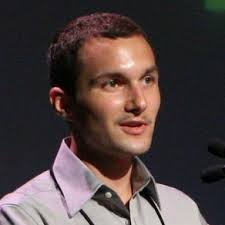
\includegraphics[scale=.60]{jeremy}  
  \begin{itemize}
    \item December 2009 - Jeremy Ashkenas first git commit
      \pause
    \item First version written in Ruby
      \pause
    \item February 2010 - Ruby version replaced by self-hosting
      implementation
      \pause
    \item Jeremy also created Backbone and Underscore
  \end{itemize}  
\end{frame}



\begin{frame}
  \frametitle{Why CoffeeScript?}
  \begin{itemize}
    \pause
    \item A language that takes out the frustrating and overly verbose bits of JS, and provides a safer, briefer way to stick to the good parts.
      \pause
    \item Syntax
    \pause
    \item ES6 Now!
  \end{itemize}
\end{frame}

\begin{frame}
  \frametitle{Why Not?}
  \begin{itemize}
    \pause
    \item Syntax
    \pause
    \item Abstraction (Not another GWT!)
    \pause
    \item Compilation
    \pause
    \item Debugging
      \pause
  \end{itemize}
\end{frame}


% \inputminted{csharp}{hello.cs}

\begin{frame}
  \frametitle{Plenty of Sugar}
  
\includegraphics[scale=.40]{sugar}
%
% TODO - consider using columns for better appearance
%
  \begin{itemize}
    \item Multi-line strings (heredoc)
    \item String interpolation
    \item Default arguments
    \item Existential operator
    \item Splats
    \item Object literals
    \item Fat arrow
    \item Prototype and this alias
    \item Classes
  \end{itemize}
\end{frame}

\begin{frame}[fragile]
  \frametitle{Function Definitions}

  \begin{minted}[lineos=false,fontsize=\normalsize]{coffeescript}
    inc = (a) ->
      a + 1
  \end{minted}

  \pause
  \vspace{.5cm}
  Compiles to:
  \vspace{.5cm}

  \begin{minted}[lineos=false,fontsize=\normalsize]{javascript}
    var inc;

    inc = function(a) {
      return a + 1;
    };    
  \end{minted}  
\end{frame}

\begin{frame}[fragile]
  \frametitle{String Interpolation}
 
  \begin{minted}[linenos=false,fontsize=\normalsize]{coffeescript}
    "#{name} is #{age} years old."
  \end{minted}

  \pause
  \vspace{.5cm}
  Compiles to:
  \vspace{.5cm}

  \begin{minted}[linenos=false,fontsize=\normalsize]{javascript}
    "" + name + " is " + age + " years old."
  \end{minted}  
\end{frame}

\begin{frame}
  \frametitle{Default Arguments}
  
\end{frame}

\begin{frame}
\frametitle{Variable Arguments}

\end{frame}

%
% ---- Testing for Existence ----
%
 \begin{frame}[fragile]
  \frametitle{Existential Operator}


  Testing for existence:

  \begin{minted}[lineos=false,fontsize=\normalsize]{coffeescript}
    if variable?
      console.log('variable is declared and not null')
  \end{minted}

  \pause
  \vspace{.5cm}
  Compiles to:
  \vspace{.5cm}


  \begin{minted}[lineos=false,fontsize=\normalsize]{javascript}
    if (typeof variable !== "undefined" && 
        variable !== null) {
      console.log('variable is declared and not null');
    }
  \end{minted}  
\end{frame}

%
% ----- Conditional Assigment -------
%
 \begin{frame}[fragile]
  \frametitle{Existential Operator}


  Conditional Assignment:

  \begin{minted}[lineos=false,fontsize=\normalsize]{coffeescript}
    getUserProfile = ->
      @profile ?= DB.getProfile(User.current)
  \end{minted}

  \pause
  \vspace{.5cm}
  Compiles to:
  \vspace{.5cm}

  \begin{minted}[lineos=false,fontsize=\normalsize]{javascript}
    getUserProfile = function() {
      return this.profile != null ? this.profile : 
        this.profile = DB.getProfile(User.current);
    };
  \end{minted}  
\end{frame}

 \begin{frame}[fragile]
  \frametitle{Existential Operator}


  Field Chaining:

  \begin{minted}[lineos=false,fontsize=\normalsize]{coffeescript}
    zip = User.current?.address?.zip
  \end{minted}

  \pause
  \vspace{.5cm}
  Compiles to:
  \vspace{.5cm}

  \begin{minted}[lineos=false,fontsize=\normalsize]{javascript}
    var zip, _ref, _ref1;

    zip = (_ref = User.current) != null ? 
      (_ref1 = _ref.address) != null ? _ref1.zip : 
      void 0 : void 0;
  \end{minted}  
\end{frame}

 \begin{frame}[fragile]
  \frametitle{Existential Operator}

  Conditional function invocation:

  \begin{minted}[lineos=false,fontsize=\normalsize]{coffeescript}
    someFunction?()
  \end{minted}

  \pause
  \vspace{.5cm}
  Compiles to:
  \vspace{.5cm}

  \begin{minted}[lineos=false,fontsize=\normalsize]{javascript}
    if (typeof someFunction === "function") {
      someFunction();
    }
  \end{minted}  
\end{frame}

\begin{frame}
  \frametitle{Heredoc}
  \inputminted{coffeescript}{src/heredoc.coffee}
\end{frame}

\begin{frame}
  \frametitle{Heredoc with interpolation}
  \inputminted{coffeescript}{src/heredoc_interp.coffee}
\end{frame}

\begin{frame}[fragile]
  \frametitle{Embedding Raw JavaScirpt}
  \begin{minted}[lineos=false,fontsize=\Large]{coffeescript}
    rawJS = `function() {
      return someComplexThing;
    }`
  \end{minted}
\end{frame}


\begin{frame}
  \frametitle{Tooling}
    
\includegraphics[scale=.40]{tooling}
  \begin{multicols}{2}
  \begin{itemize}
    \item Intellij/Rubymine
    \item Emacs
    \item Vim
    \item Sublime
    \item node
    \item \href{http://www.coffeelint.org/}{CoffeLint}
    \item Rails
    \item \href{http://www.playframework.com/documentation/2.0/AssetsCoffeeScript}{Play}
    \item Eclipse
    \item \href{https://jawr.java.net/}{Jawr}
    \item
      \href{http://www.html5rocks.com/en/tutorials/developertools/sourcemaps/}{Source
      Maps}

  \end{itemize}
\end{multicols}
\end{frame}

\end{document}
